
\documentclass[
	a4paper, 
	10pt,
	unnumberedsections, 
	twoside,
]{LTJournalArticle}

\addbibresource{sample.bib}

\runninghead{Shortened Running Article Title} 

\footertext{\textit{Journal of Biological Sampling} (2024) 12:533-684} 

\setcounter{page}{1} 

\title{An Article Title That Spans Multiple\\ Lines to Show Line Wrapping} % A
\author{%
	John Smith\textsuperscript{1,2}, Robert Smith\textsuperscript{3} and Jane Smith\textsuperscript{1}\thanks{Corresponding author: \href{mailto:jane@smith.com}{jane@smith.com}\\ \textbf{Received:} October 20, 2023, \textbf{Published:} December 14, 2023}
}

\date{\footnotesize\textsuperscript{\textbf{1}}School of Chemistry, The University of Michigan\\ \textsuperscript{\textbf{2}}Physics Department, The University of Wisconsin\\ \textsuperscript{\textbf{3}}Biological Sciences Department, The University of Minnesota}

\renewcommand{\maketitlehookd}{%
	\begin{abstract}
		\noindent Lorem ipsum dolor sit amet, consectetur adipiscing elit. Praesent porttitor arcu luctu Sed non pretium nibh. Donec cursus maximus luctus. Vivamus lobortis eros et massa porta porttitor.
	\end{abstract}
}

\begin{document}

\maketitle 

\section{Introduction}

Lorem ipsuma volutpat velit condimentum convallis et facilisis dolor.

\begin{equation}
	\cos^3 \theta =\frac{1}{4}\cos\theta+\frac{3}{4}\cos 3\theta
	\label{eq:example}
\end{equation}

Automatically referencing an equation number using its label: Equation \ref{eq:example}.

In hac haidunt dignissim egestas.

%------------------------------------------------

\section{Methodologies}

\subsection{Sample Sites \& Processing}

This line shows how to use explain or cite text\footnote{Example footnote text.}.

This is a bullet point list:

\begin{itemize}
	\item Arcu eros accumsan sapien tortor non nisi
	\item Pellentesque bibendum pretium aliquet
\end{itemize}

Mauris interdum portticonvallis pellentesque.

This is a numbered list:

\begin{enumerate}
	\item Donec dolor arcu, rutrum id molestie in, viverra sed diam
	\item Curabitur feugiat
	\item Turpis sed auctor facilisis
\end{enumerate}

\subsection{Species Identification}

Proin loallis pellentesque.

\subsection{Data Analysis}

Vestibulut. In et ipsum libero. Nullam tempor ligula a massa convallis pellentesque.



\section{Results}

\begin{table} 
	\caption{Example single column table.}
	\centering
	\begin{tabular}{l l r}
		\toprule
		\multicolumn{2}{c}{Location} \\
		\cmidrule(r){1-2}
		East Distance & West Distance & Count \\
		\midrule
		100km & 200km & 422 \\
		350km & 1000km & 1833 \\
		600km & 1200km & 890 \\
		\bottomrule
	\end{tabular}
	\label{tab:distcounts}
\end{table}

Referencing a table using its label: Table \ref{tab:distcounts}.

\begin{table*} 
	\caption{Example two column table with fixed-width columns.}
	\centering
	\begin{tabular}{L{0.2\linewidth} L{0.2\linewidth} R{0.15\linewidth}} 
		\toprule
		\multicolumn{2}{c}{Location} \\
		\cmidrule(r){1-2}
		East Distance & West Distance & Count \\
		\midrule
		100km & 200km & 422 \\
		350km & 1000km & 1833 \\
		600km & 1200km & 890 \\
		\bottomrule
	\end{tabular}
\end{table*}

Aenean feugiat pellentesque venenatis. Sed faucibus tristique tortor vel ultrices. Donec cotrum sagittis dui. Donec non est a metus varius finibus. Pellentesque rutrum pellentesque ligula, vitae accumsan nulla hendrerit ut.

\begin{figure} 
	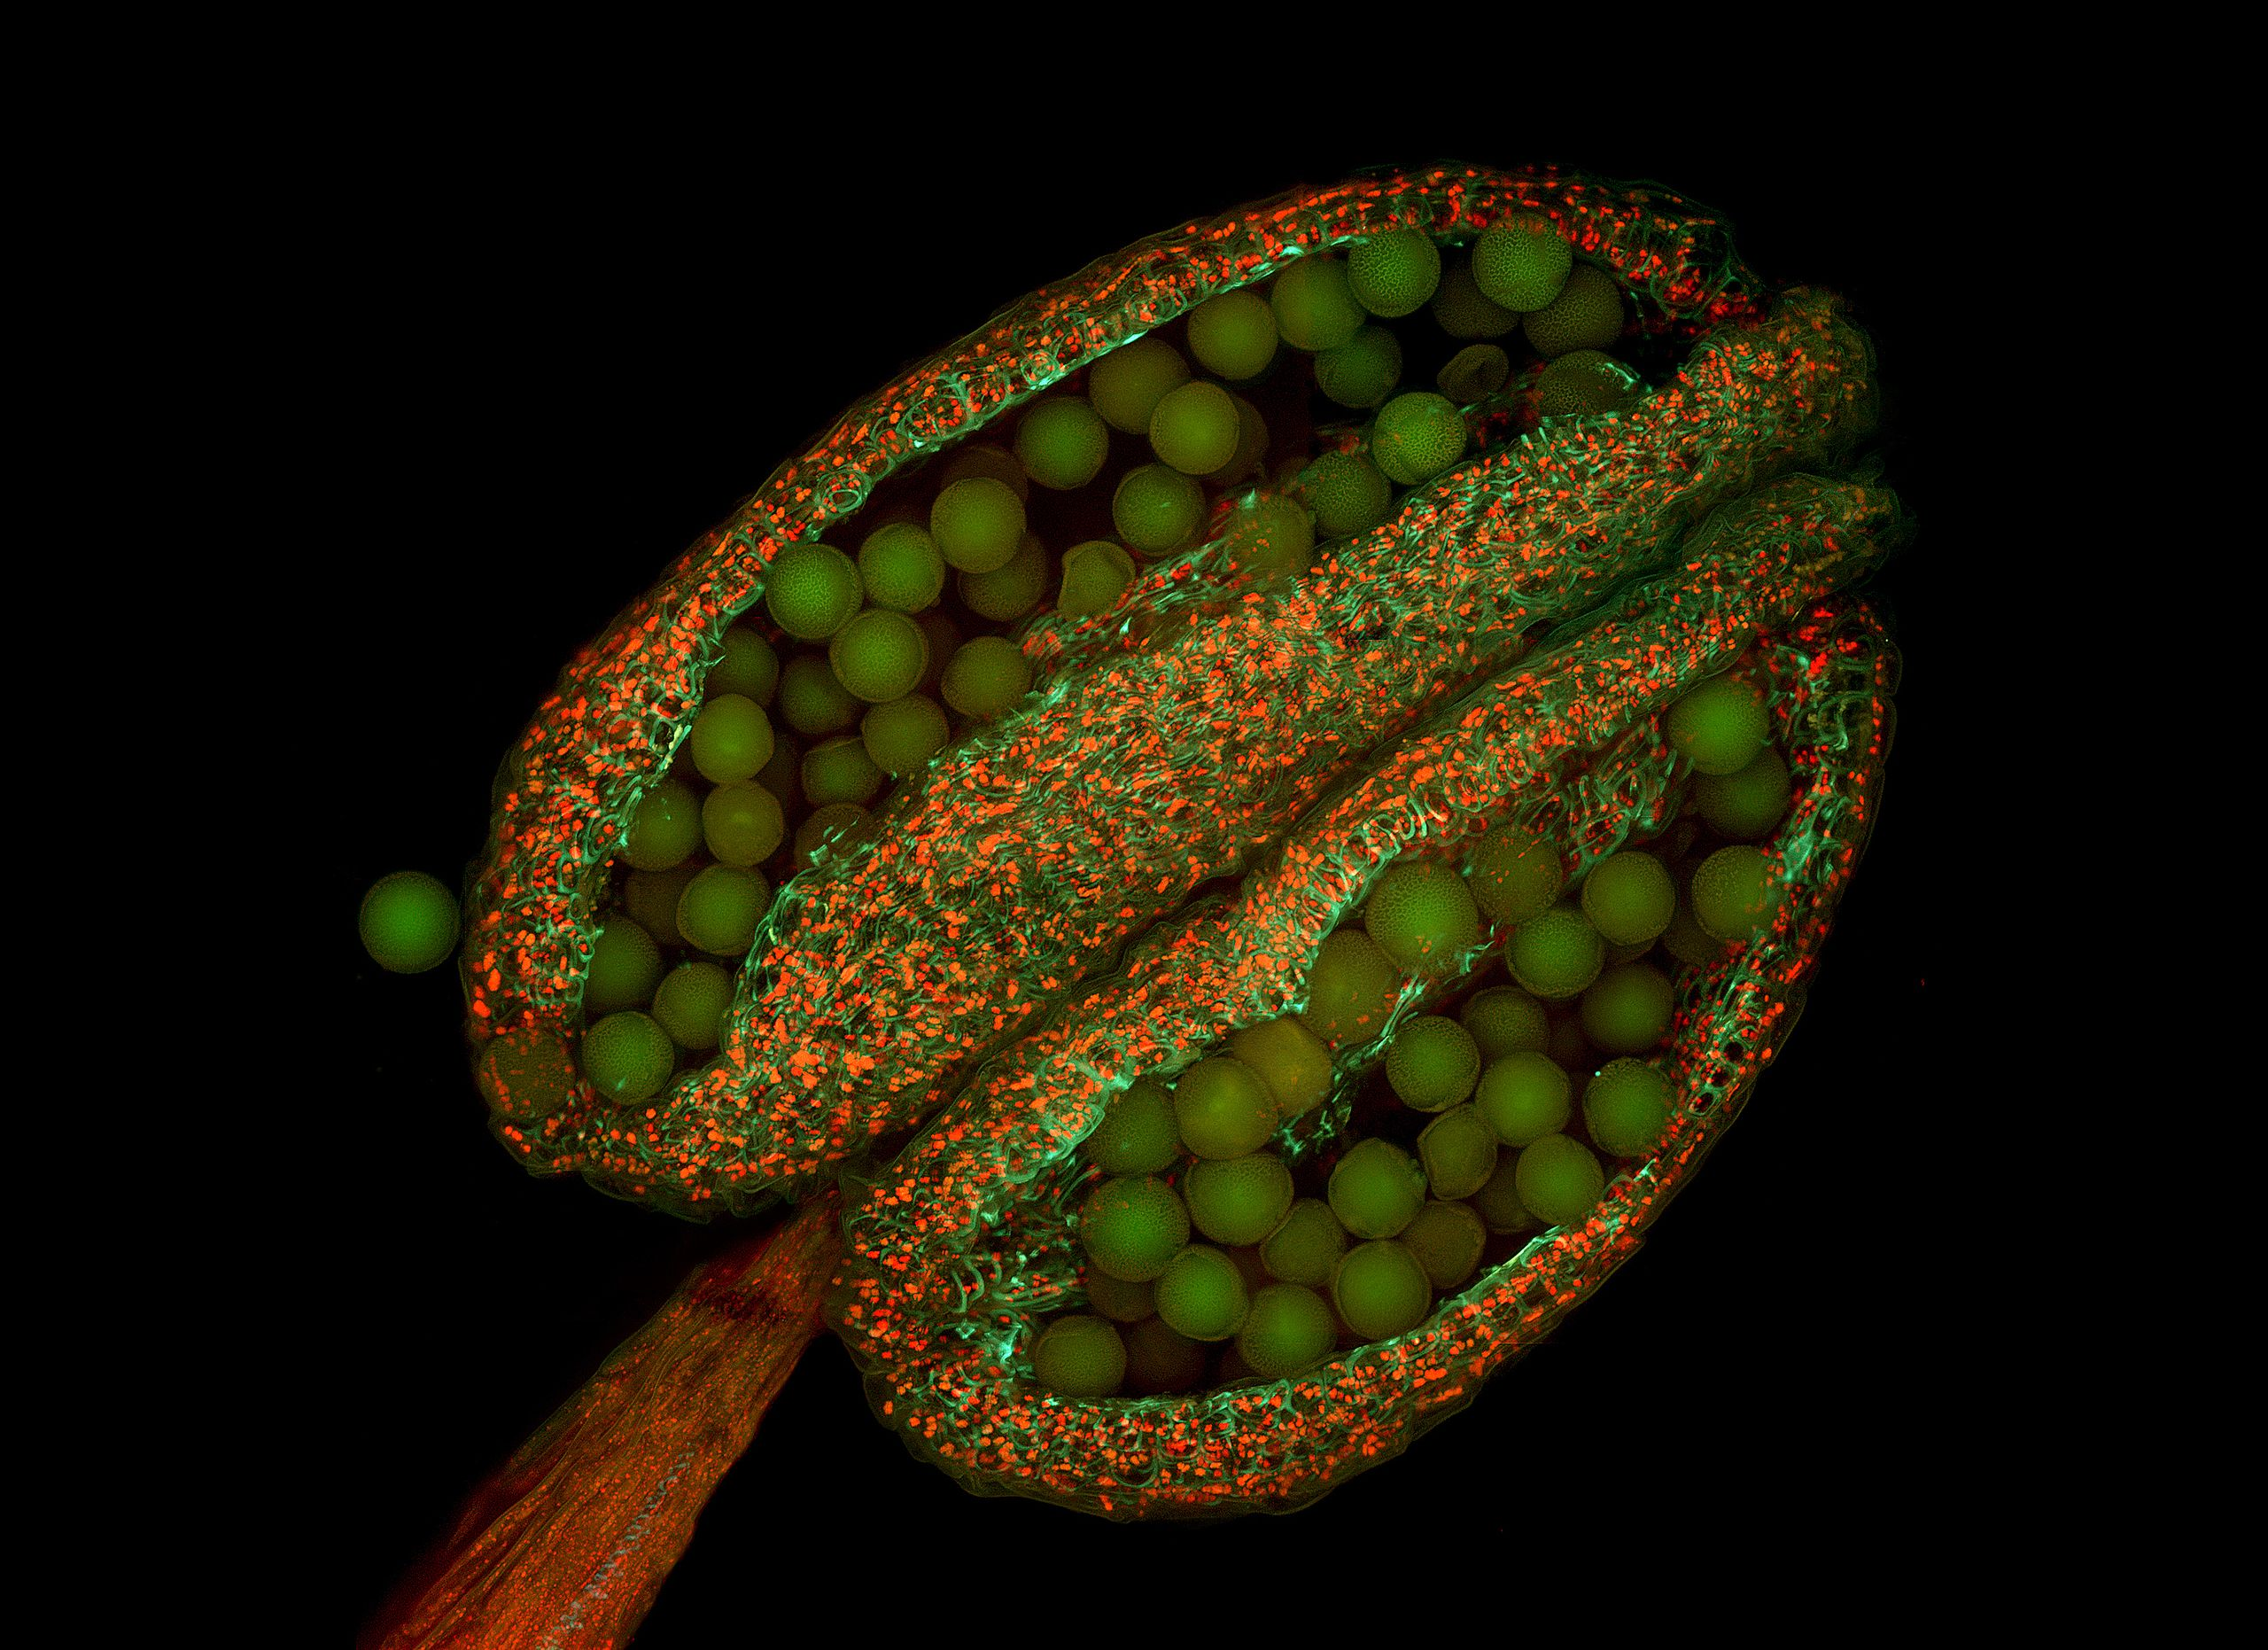
\includegraphics[width=\linewidth]{Tolmukapea.jpg}
	\caption{Anther of thale cress (Arabidopsis thaliana), fluorescence micrograph. Source: Heiti Paves, \href{https://commons.wikimedia.org/wiki/File:Tolmukapea.jpg}{https://commons.wiki-\\media.org/wiki/File:Tolmukapea.jpg}.}
	\label{fig:tcanther}
\end{figure}   

Referencing a figure using its label: Figure \ref{fig:tcanther}.

Aenean porttitor bh.

\begin{figure*} % Two column figure (notice the starred environment)
	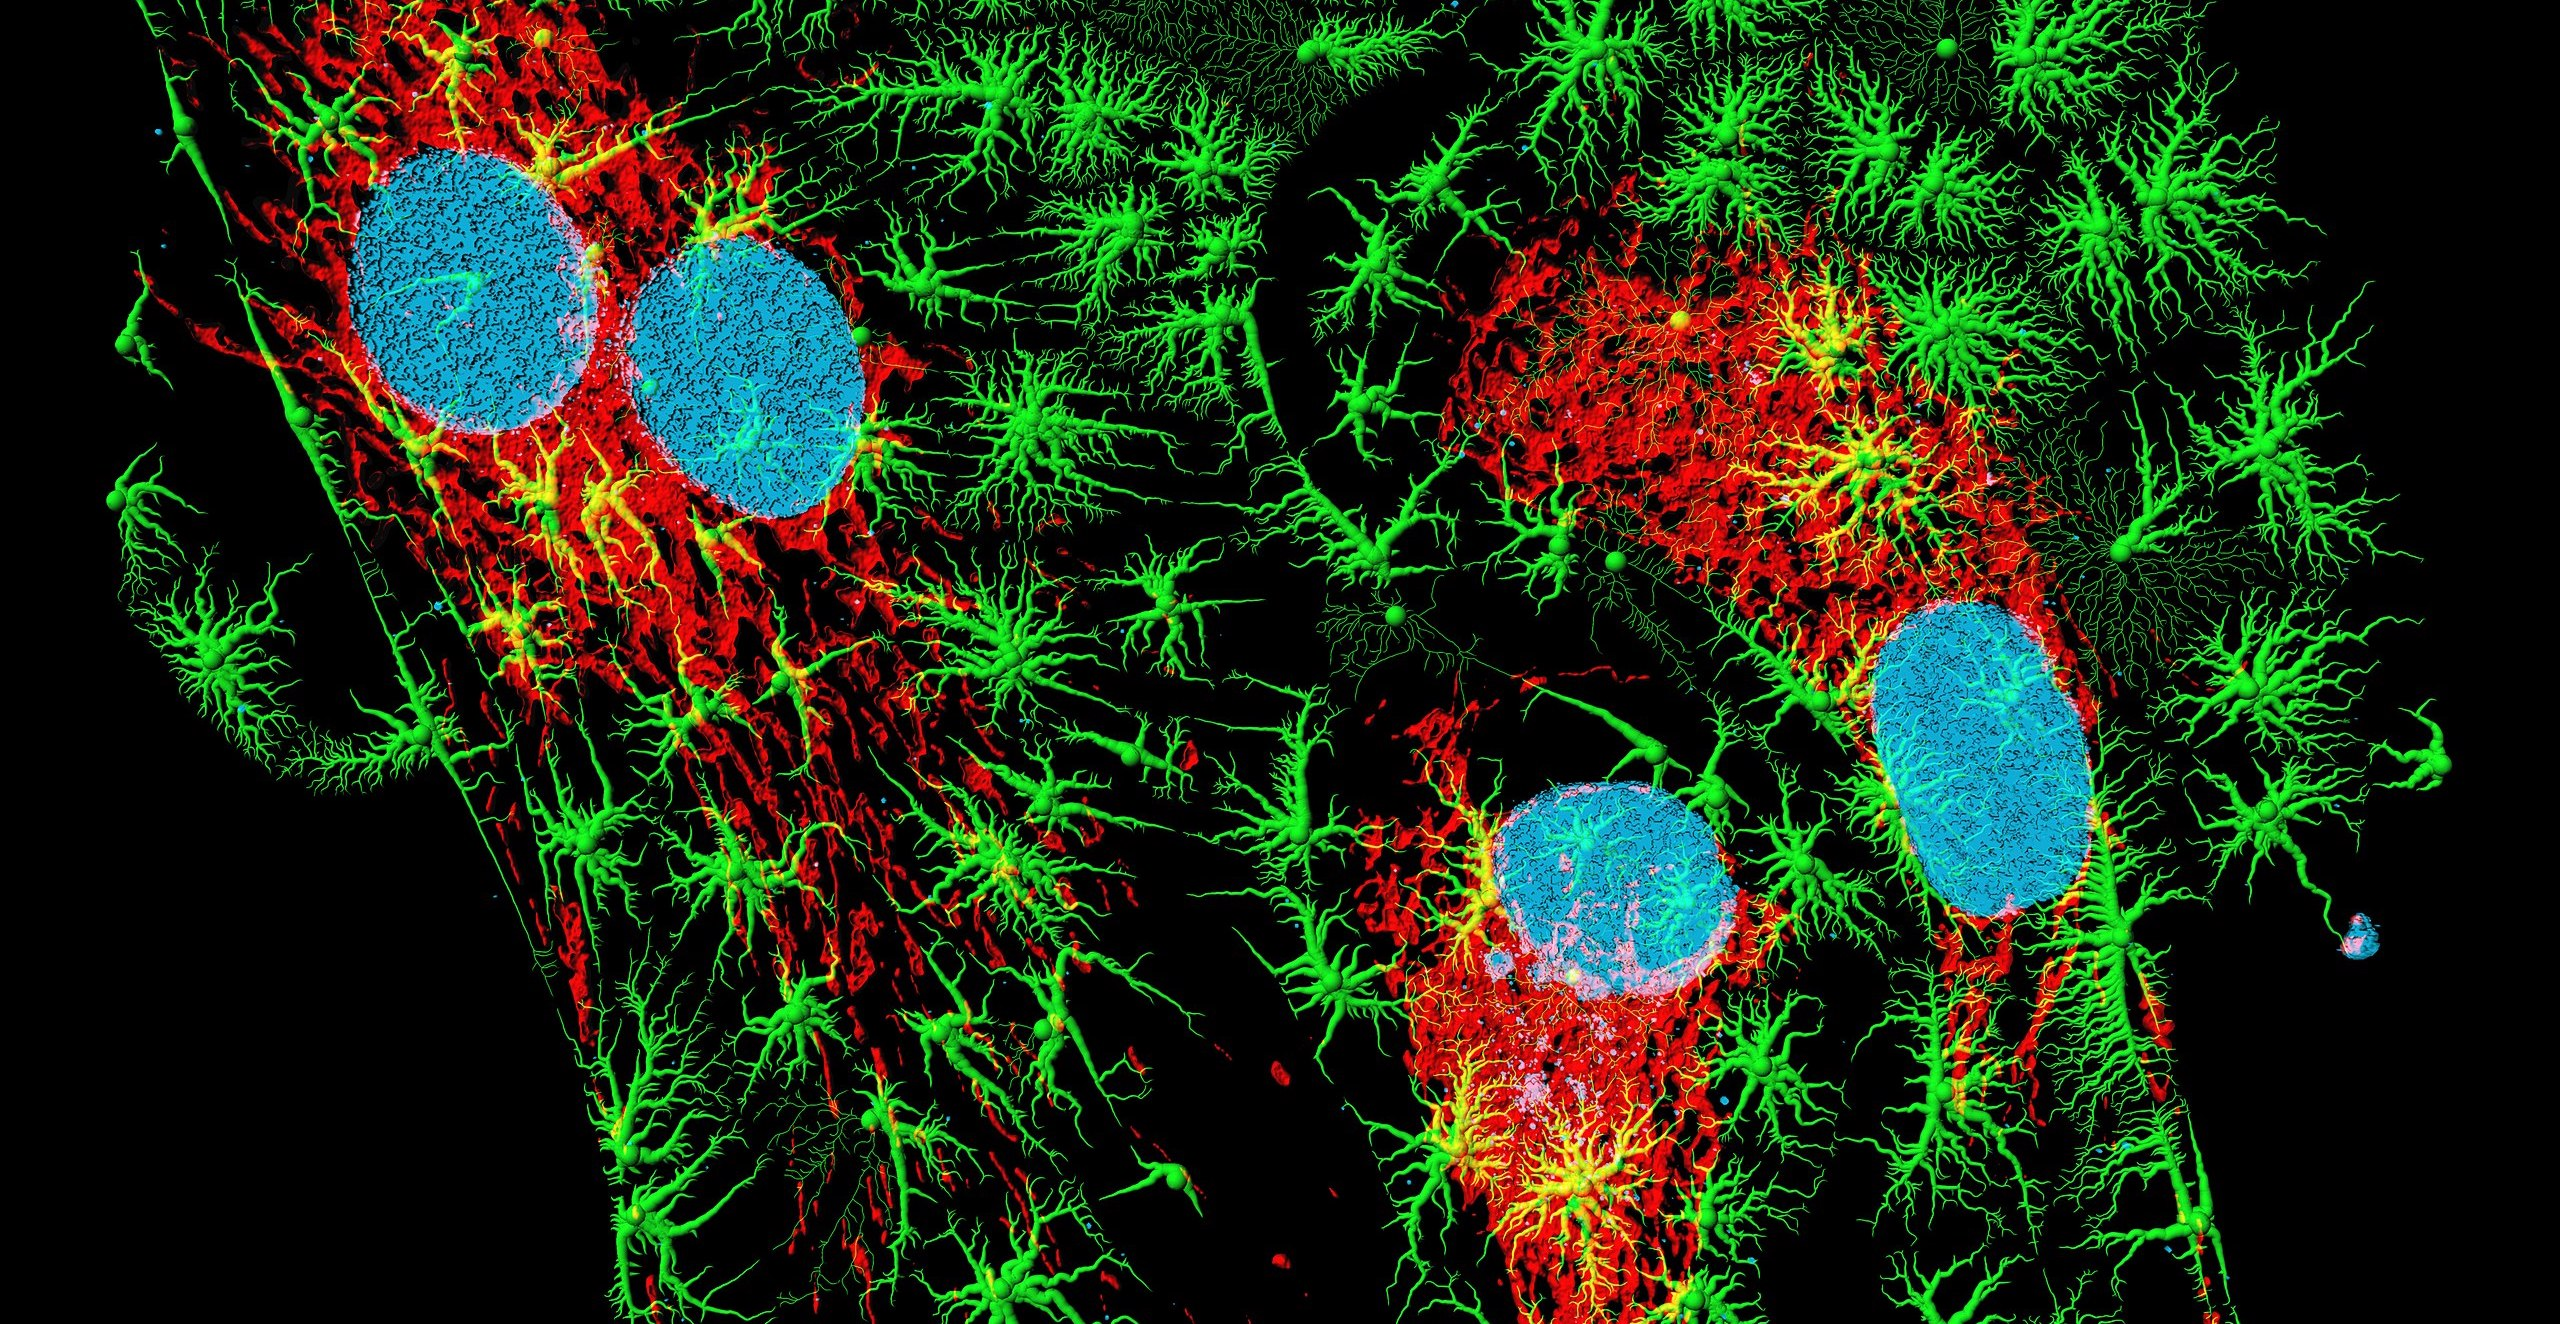
\includegraphics[width=\linewidth]{Fibroblastid.jpg}
	\caption{Bovine pulmusing fluorescent marker dyes. Source: Heiti Paves, \href{https://commons.wikimedia.org/wiki/File:Fibroblastid.jpg}{https://commons.wikimedia.org/wiki/File:Fibroblastid.jpg}.}
	\label{fig:bpartery}
\end{figure*}

Orci varius natoque penatibus et magnis dis parturient montes, nascetur ridiculus mus. st porttitor cursus. Cras placerat faucibus nunc, a laoreet justo dignissim sit amet.

\subsection{International Support}

\noindent àáâäãåèéêëìíîïòóôöõøùúûüÿýñçčšž

\noindent ÀÁÂÄÃÅÈÉÊËÌÍÎÏÒÓÔÖÕØÙÚÛÜŸÝÑ

\noindent ßÇŒÆČŠŽ

\subsection{Links}

This is a clickable URL link: \href{https://www.latextemplates.com}{LaTeX Templates}. This is a clickable email link: \href{mailto:vel@latextemplates.com}{vel@latextemplates.com}. This is a clickable monospaced URL link: \url{https://www.LaTeXTemplates.com}.

\section{Discussion}

This statement requires citation \autocite{Smith:2023qr}. This statement requires multiple citations \autocite{Smith:2023qr, Smith:2024jd}. This statement contains an in-text citation, for directly referring to a citation like so: \textcite{Smith:2024jd}.

\subsection{Subsection One}

Suspendisse potenti. Vivamus et vel ex. Nunc maximus quam orci, quis pulvinar nibh eleifend ac. Quisque consequat lacus magna, eu posuere tellus iaculis ac. Sed vitae tortor tincidunt ante sagittis iaculis.

\subsection{Subsection Two}

Nullam mollis tellus lorem, sed congue ipsum euismod a. Donec pulvinar neque sed ligula ornare sodales. Null

\subsubsection{Subsubsection Example}

Duis venenatis eget lectus a aliquet. Integer vulputate ante suscipit felis feugiat rutrum. Aliquam eget dolor eu augue elementum ornare. Nulla fringilla interdum volutpat. Sed tincidunt,  aliquet turpis. Vivamus molestie urna quis tempor tristique. Proin hendrerit sem nec tempor sollicitudin.



\printbibliography % Output the bibliography


\end{document}
